\section{eo\-Truncated\-Select\-Many$<$ EOT $>$ Class Template Reference}
\label{classeo_truncated_select_many}\index{eoTruncatedSelectMany@{eoTruncatedSelectMany}}
eo\-Truncated\-Select\-Many selects many individuals using {\bf eo\-Select\-One}{\rm (p.\,\pageref{classeo_select_one})} as it's mechanism.  


{\tt \#include $<$eo\-Truncated\-Select\-Many.h$>$}

Inheritance diagram for eo\-Truncated\-Select\-Many$<$ EOT $>$::\begin{figure}[H]
\begin{center}
\leavevmode
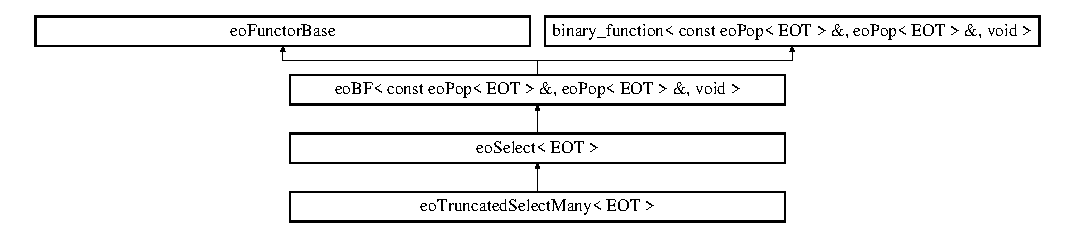
\includegraphics[height=2.75184cm]{classeo_truncated_select_many}
\end{center}
\end{figure}
\subsection*{Public Member Functions}
\begin{CompactItemize}
\item 
{\bf eo\-Truncated\-Select\-Many} ({\bf eo\-Select\-One}$<$ {\bf EOT} $>$ \&\_\-select, double \_\-rate\-Genitors, double \_\-rate\-Fertile, bool \_\-interpret\_\-as\_\-rate\-G=true, bool \_\-interpret\_\-as\_\-rate\-F=true)\label{classeo_truncated_select_many_a0}

\begin{CompactList}\small\item\em Ctor. \item\end{CompactList}\item 
{\bf eo\-Truncated\-Select\-Many} ({\bf eo\-Select\-One}$<$ {\bf EOT} $>$ \&\_\-select, {\bf eo\-How\-Many} \_\-how\-Many\-Genitors, {\bf eo\-How\-Many} \_\-how\-Many\-Fertile)\label{classeo_truncated_select_many_a1}

\item 
virtual void {\bf operator()} (const {\bf eo\-Pop}$<$ {\bf EOT} $>$ \&\_\-source, {\bf eo\-Pop}$<$ {\bf EOT} $>$ \&\_\-dest)
\begin{CompactList}\small\item\em The implementation repeatidly selects an individual. \item\end{CompactList}\end{CompactItemize}
\subsection*{Private Attributes}
\begin{CompactItemize}
\item 
{\bf eo\-Select\-One}$<$ {\bf EOT} $>$ \& {\bf select}\label{classeo_truncated_select_many_r0}

\item 
{\bf eo\-How\-Many} {\bf how\-Many\-Genitors}\label{classeo_truncated_select_many_r1}

\item 
{\bf eo\-How\-Many} {\bf how\-Many\-Fertile}\label{classeo_truncated_select_many_r2}

\end{CompactItemize}


\subsection{Detailed Description}
\subsubsection*{template$<$class EOT$>$ class eo\-Truncated\-Select\-Many$<$ EOT $>$}

eo\-Truncated\-Select\-Many selects many individuals using {\bf eo\-Select\-One}{\rm (p.\,\pageref{classeo_select_one})} as it's mechanism. 

Therefore {\bf eo\-Select\-Many}{\rm (p.\,\pageref{classeo_select_many})} needs an {\bf eo\-Select\-One}{\rm (p.\,\pageref{classeo_select_one})} in its ctor

It will use an eo\-How\-Mnay to determine the number of guys to select, and push them to the back of the destination population.

And it will only perform selection from the top guys in the population.

It is NOT a special case of {\bf eo\-Select\-Many}{\rm (p.\,\pageref{classeo_select_many})} because it needs to SORT the population to discard the worst guys before doing the selection

However, the same result can be obtained by embedding an {\bf eo\-Truncated\-Select\-One}{\rm (p.\,\pageref{classeo_truncated_select_one})} into an {\bf eo\-Select\-Many}{\rm (p.\,\pageref{classeo_select_many})} ... 



Definition at line 53 of file eo\-Truncated\-Select\-Many.h.

\subsection{Member Function Documentation}
\index{eoTruncatedSelectMany@{eo\-Truncated\-Select\-Many}!operator()@{operator()}}
\index{operator()@{operator()}!eoTruncatedSelectMany@{eo\-Truncated\-Select\-Many}}
\subsubsection{\setlength{\rightskip}{0pt plus 5cm}template$<$class EOT$>$ virtual void {\bf eo\-Truncated\-Select\-Many}$<$ {\bf EOT} $>$::operator() (const {\bf eo\-Pop}$<$ {\bf EOT} $>$ \& {\em \_\-source}, {\bf eo\-Pop}$<$ {\bf EOT} $>$ \& {\em \_\-dest})\hspace{0.3cm}{\tt  [inline, virtual]}}\label{classeo_truncated_select_many_a2}


The implementation repeatidly selects an individual. 

\begin{Desc}
\item[Parameters:]
\begin{description}
\item[{\em \_\-source}]the source population \item[{\em \_\-dest}]the resulting population (size of this population is the number of times {\bf eo\-Select\-One}{\rm (p.\,\pageref{classeo_select_one})} is called. It empties the destination and adds the selection into it) \end{description}
\end{Desc}


Implements {\bf eo\-BF$<$ const eo\-Pop$<$ EOT $>$ \&, eo\-Pop$<$ EOT $>$ \&, void $>$} {\rm (p.\,\pageref{classeo_b_f_a1})}.

Definition at line 77 of file eo\-Truncated\-Select\-Many.h.

References eo\-Select\-One$<$ EOT, Worth\-T $>$::setup(), eo\-Pop$<$ EOT $>$::shuffle(), and eo\-Pop$<$ EOT $>$::sort().

The documentation for this class was generated from the following file:\begin{CompactItemize}
\item 
eo\-Truncated\-Select\-Many.h\end{CompactItemize}
